
\section{State dependent discontinuity problem}
In this Section, we model the state dependent discontinuity problem. We start by noting that this problem cannot be solved using the discontinuity handling used in the previous problem as we do not when the discontinuity will happen. This problem also has more discontinuity than the previous problem and as such is a harder problem that even error-controlled solvers will not be able to solve. We will also show that it cannot be solved simply by sharpening the tolerance and using an error-control solver as it was the case in the previous problem.
 
As in Section $\ref{section:time_problem}$, changes in the modelling parameter $\beta$ introduce discontinuities in the function $f(t, y)$ and thus some solvers will crash when trying to solve them. This problem is harder than the time dependent discontinuity in that there are more discontinuities because the parameter will be toggled more than once as we solve for a longer time period.

This problem will also allow longer term forecasts and will model the 'waves' of the pandemic. It uses a state variable, the number of Exposed people, E, to change the parameter $\beta$. When the number of exposed people is greater or equal to 25000,  measures will be introduced and thus $\beta$ will change from 0.9 to 0.005. When the number of exposed people drops back to 10000, the government will relax the measures again and $\beta$ becomes 0.9 again. We run this over a longer time period to see several waves of the virus. We also note that the problem is unstable when $\beta$ is 0.9 but is stable when $beta$ is 0.005.

Because we do not know beforehand at what times the discontinuity will occur, this problem cannot be solved by using cold starts as we have done before. We thus start off with a naive treatment of the problem with if-statements inside the function and show how this will never lead to the correct solution. We proceed to show how the problem cannot be solved even at sharp tolerance and finally we will introduce a way to efficiently and accurately solve it using event detection.

For the sections on the state dependent problem, we graph the number of Exposed people, E, rather than the number of infected people, I. This is because we are toggling the parameter $\beta$ based on the value of E and graphing E will reflect that.

\subsection{Naive treatment of Covid-19 state discontinuity model}
\label{subsection:naive_state_problem}
The naive treatment of this problem is to use global variables or parameters for whether measures are implemented or not and to toggle them as we reach the required thresholds. Global variables are needed because we need to know if the number of Exposed people is going up or down to know whether we need to check for the maximum or the minimum threshold.

We then have an if-statement which will choose the value of parameter $\beta$ based on whether measures are implemented. We will show that this naive implementation will lead to huge discrepancies in the solvers' results. The pseudo-code for this problem thus looks as such:

\begin{minipage}{\linewidth}
\begin{lstlisting}[language=Python]
measures_implemented = False
direction = "up"
function model_with_if(_, y):
    (S, E, I, R) = y
    global measures_implemented, direction
    if (direction == "up"):
        if (E > 25000):
            measures_implemented = True
            direction = "down"
    else:
        if (E < 10000):
            measures_implemented = False
            direction = "up"

    if measures_implemented:
        beta = 0.005 
    else:
        beta = 0.9
    // code to get (dSdt, dEdt, dIdt, dRdt)
    return (dSdt, dEdt, dIdt, dRdt)
\end{lstlisting}
\end{minipage}

\subsubsection{State Discontinuity in R}
\begin{figure}[h]
	\centering
	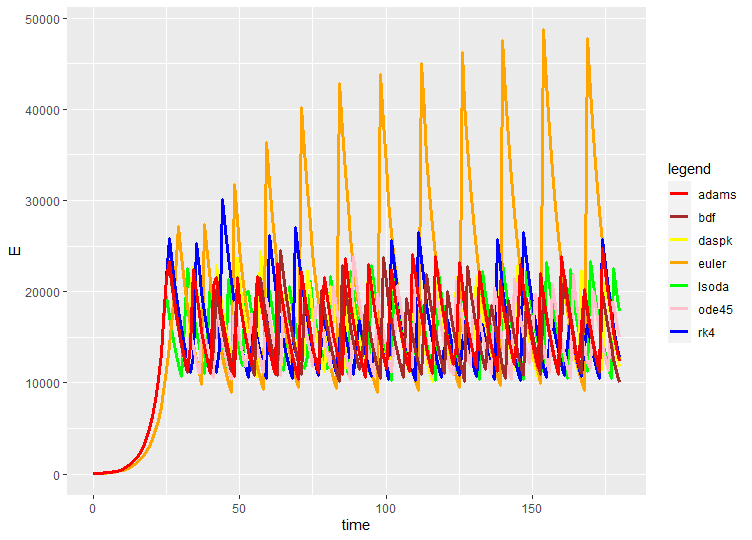
\includegraphics[width=0.7\linewidth]{./figures/state_discontinuity_R}
	\caption{State Discontinuity in R}
	\label{fig:state_discontinuity_R}
\end{figure}
Figure $\ref{fig:state_discontinuity_R}$ shows how difficult this problem is with a naive treatment. We note that none of the solutions are aligned and also that none of the solvers has the correct solution that we will introduce in Section $\ref{subsection:state_with_event_detection}$. We note that all the solvers, even the error controlled ones, did not issue a warning or any flag about the integration and thus researchers may be tempted to think that any of them is accurate. In solving this problem thus, the solvers all had their error estimation algorithms wrongly satisfy the tolerance. 

As we are modelling E and not I, we expect that the graph goes from 25000 to 10000 and back to 25000 repeatedly but none of these graphs do so in the required pattern. We would also expect the solvers that have error control to repeatedly reduce the step-size to satisfy the tolerance and align with each others but Figure $\ref{fig:state_discontinuity_R}$ shows that these solvers did not perform enough error control; their tolerances were satisfied at wrong answers and thus the error estimation algorithm did not work as expected.

We also note that the result for 'euler' is especially bad as it even reaches 40000. This is again as expected as 'euler' has no error control; 'rk4', the other fixed step-size method, is also performing terribly as we see it reach 30000 in its third peak. This is all despite the fact that the space between the points is as small as it was when performing the first experiment.

Another important fact to note is how poorly 'radau', as shown in Figure $\ref{fig:state_discontinuity_radau_R}$, is performing. This is not a problem in the R programming environment as similar results will be seen in Python in the next section and in the Fortran code. We will discuss our findings on 'radau' in Section $\ref{section:fortran_inaccuracies}$.

\begin{figure}[h]
	\centering
	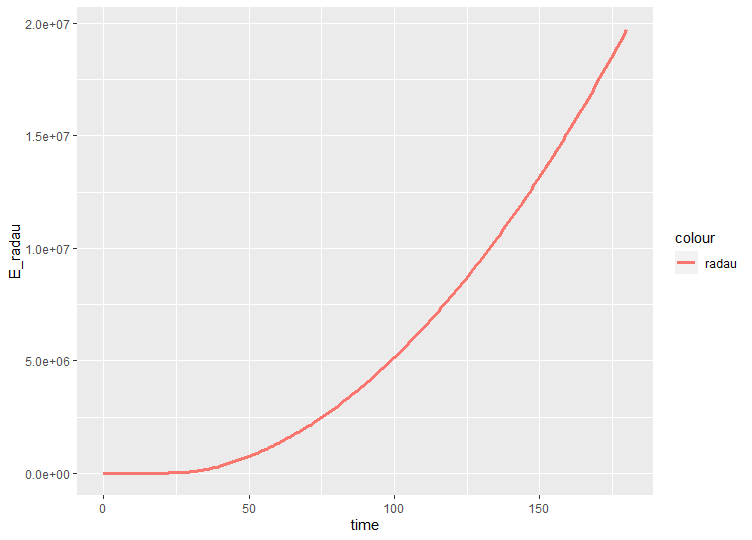
\includegraphics[width=0.7\linewidth]{./figures/state_discontinuity_radau_R}
	\caption{State Discontinuity of Radau in R}
	\label{fig:state_discontinuity_radau_R}
\end{figure}

We then proceed to show that sharp tolerances and thus more stringent error control are not enough to solve this problem as it was for the time dependent discontinuity problem. We repeated the experiment at the sharpest tolerance usable before some of the solvers cannot integrate which was at $10^{-13}$. We set both the absolute and relative tolerance to that number and the results are shown in Figure $\ref{fig:state_discontinuity_sharp_R}$.

\begin{figure}[h]
	\centering
	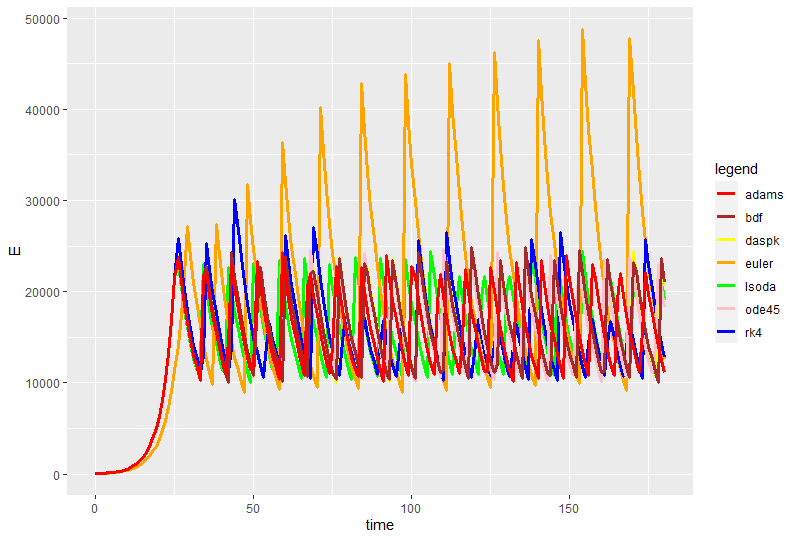
\includegraphics[width=0.7\linewidth]{./figures/state_discontinuity_sharp_R}
	\caption{State Discontinuity in R at high tolerances}
	\label{fig:state_discontinuity_sharp_R}
\end{figure}

We can see from Figure $\ref{fig:state_discontinuity_sharp_R}$ that the situation has only marginally improved. None of the solvers are on the same line and none of them cleanly oscillate between 10000 and 25000. We note that the error-controlled solvers are following the correct pattern and that until about time 20-30, some of them are along the same line showing that error-control might be able to step over one state dependent discontinuity.

The fixed step-size method 'euler' still gets results that are far off and 'rk4' is far off at the start but follows a decent pattern at the end. This surprisingly good performance of 'rk4' is again due to the fact that it has a small initial step-size as its step-size depends on the set of output points.

We can also point out that at such sharp tolerances, 'radau' is no longer having the abnormal behaviour we saw previously. From Figure $\ref{fig:state_discontinuity_radau_sharp_R}$, we can see that it oscillates between 10000 and 25000 as it should but this is still not quite the correct answer as we will discuss in Section $\ref{subsection:state_with_event_detection}$. From supplementary experiments 'radau' starts performing correctly at about a tolerance of $10^{-9}$.

\begin{figure}[h]
	\centering
	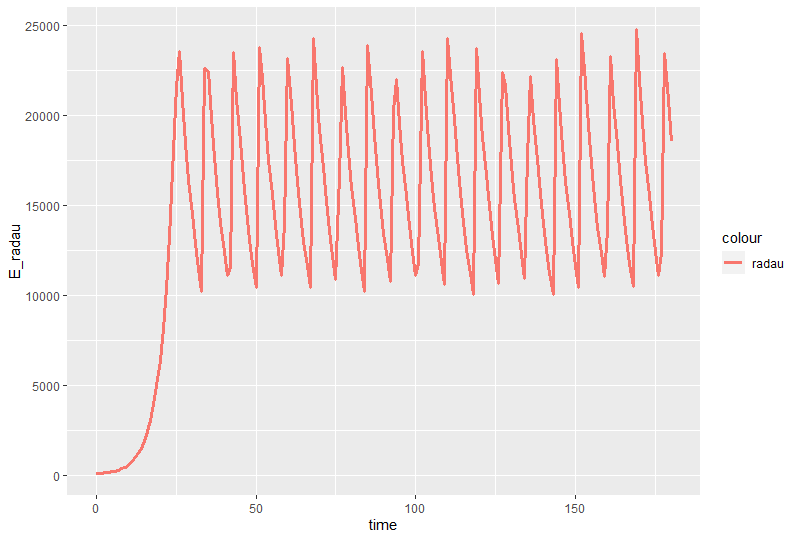
\includegraphics[width=0.7\linewidth]{./figures/state_discontinuity_sharp_radau_R}
	\caption{State Discontinuity of Radau in R at high tolerances}
	\label{fig:state_discontinuity_radau_sharp_R}
\end{figure}

\subsubsection{State discontinuity in Python}
We also perform the experiment with if-statements and global variables in Python with equally inaccurate results.

\begin{figure}[h]
	\centering
	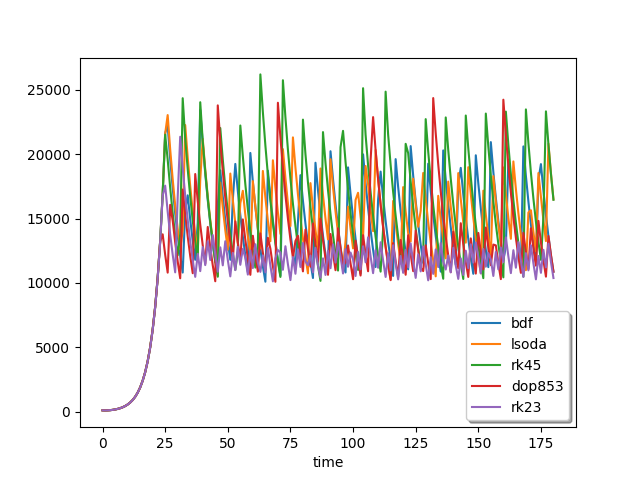
\includegraphics[width=0.7\linewidth]{./figures/state_discontinuity_py}
	\caption{State Discontinuity in Python}
	\label{fig:state_discontinuity_python}
\end{figure}
Figure $\ref{fig:state_discontinuity_python}$ shows what happens when the problem is coded with global variables and if-statements in Python. We can see that the results are similar to those in R. This is despite the fact that all solvers in Python have error control.

We note that all the solvers expect 'RK23' at least oscillate between 10000 and 25000 though in completely random patterns. They have their peak and troughs at different times and no warnings or flags were set showing that the solvers' error estimation algorithm were wrongly satisfied with these results.

The 'RK23' solver, in purple, has a completely different pattern as the other solvers.  It never reaches 25000 and only oscillates between around 10000 and 15000. 

VI ===========================
I DONT KNOW WHY 'RK23' does this.
====================== VI

Again, as shown in Figure $\ref{fig:state_discontinuity_radau_py}$, 'Radau' messes up completely and grows exponentially even though the parameter $\beta$ should be set to start an exponential decay as it did with all other solvers.

\begin{figure}[h]
	\centering
	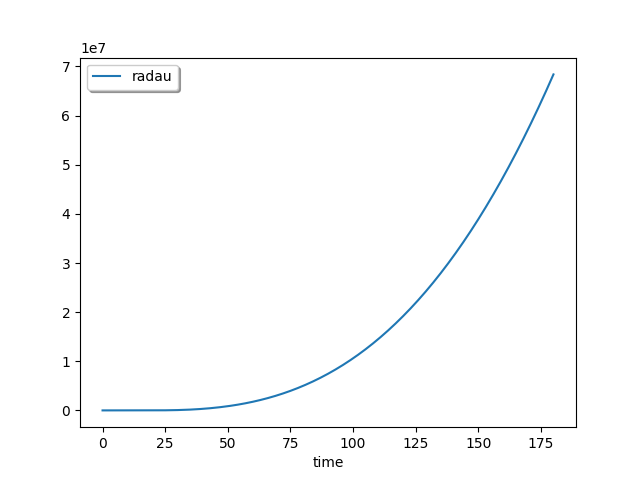
\includegraphics[width=0.7\linewidth]{./figures/state_discontinuity_radau_py}
	\caption{State Discontinuity of Radau in Python}
	\label{fig:state_discontinuity_radau_py}
\end{figure}

We then used very sharp tolerances to solve the problem but, as is the case in the R environment, none of the solvers obtained a correct solution. The highest tolerance we could use in Python without any one method failing was $10^{-12}$. Both the absolute and relative tolerance was set to that value and Figure $\ref{fig:state_discontinuity_sharp_python}$ shows the results from this sharp tolerance experiment.

\begin{figure}[h]
	\centering
	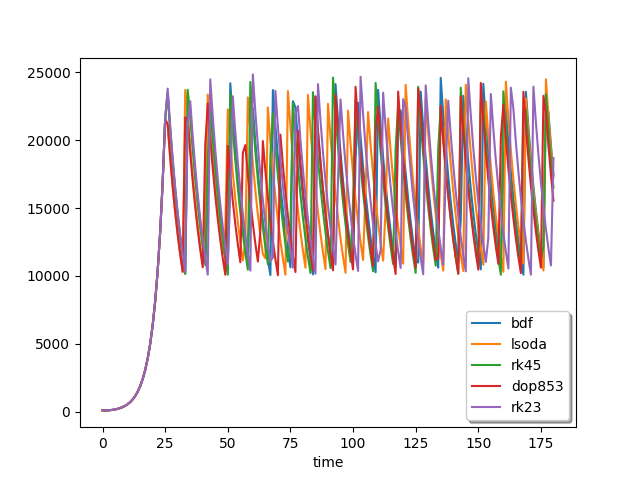
\includegraphics[width=0.7\linewidth]{./figures/state_discontinuity_sharp_py}
	\caption{State Discontinuity in Python at sharp tolerances}
	\label{fig:state_discontinuity_sharp_python}
\end{figure}

Figure $\ref{fig:state_discontinuity_sharp_python}$ shows that the solution did improve. Still, the solvers are not all on the same line. We note that none of the solvers are oscillating beyond 25000 as was the case with the fixed-step solvers in R. At sharp tolerances, the solutions are aligned for the first few discontinuities with only some blurring until about time 25 or 30. Though the pattern is correct, none of the solvers are on the same line telling us that none actually got the correct solution.

We note that 'RK23' is now following the correct pattern in that it oscillates between 10000 and 25000 whereas it only reached 15000 at the default tolerances. 

Again, as shown in Figure $\ref{fig:state_discontinuity_sharp_radau_py}$,'Radau' stops its weird behaviour at this sharp tolerances and follows the pattern we were expecting from the solution but as we will show in Section $\ref{subsection:state_with_event_detection}$, this is still not the correct solution. 'Radau' starts performing well at around a tolerance of $10^{-10}$.

We should also note that the R and Python implementation of 'Radau' are different. The 'Radau' solvers in Python is implemented in Python with the NumPy library whereas R uses the Fortran code. Thus we eliminate the possibility of a bug in the code as well as any problem stemming from the interface from R to Fortran or from Python to NumPy. The problem is simply in how the algorithm interacts with this naive implementation of the state dependent discontinuity.


\begin{figure}[h]
	\centering
	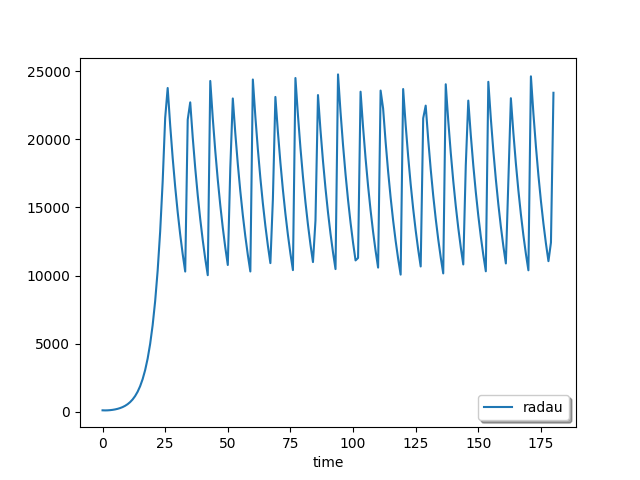
\includegraphics[width=0.7\linewidth]{./figures/state_discontinuity_sharp_radau_py}
	\caption{State Discontinuity of Radau in Python at sharp tolerances}
	\label{fig:state_discontinuity_sharp_radau_py}
\end{figure}

\subsubsection{State discontinuity in Scilab}
We perform the experiment with if-statements and global variables in Scilab and the results are as shown in Figures $\ref{fig:state_discontinuity_scilab}$ and $\ref{fig:state_discontinuity_sharp_scilab}$.

\begin{figure}[h]
	\centering
	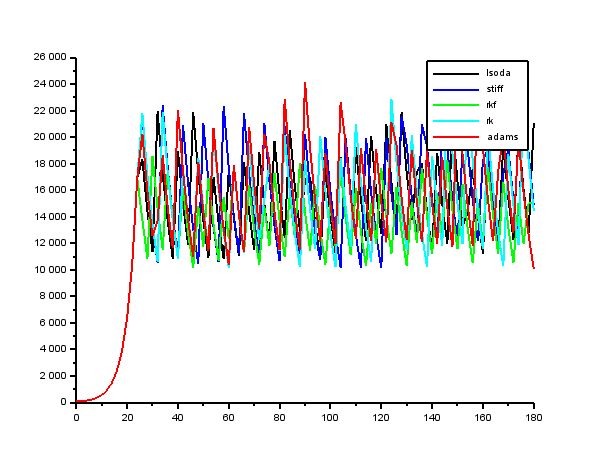
\includegraphics[width=0.7\linewidth]{./figures/state_discontinuity_scilab}
	\caption{State Discontinuity in Scilab}
	\label{fig:state_discontinuity_scilab}
\end{figure}
Figure $\ref{fig:state_discontinuity_scilab}$ shows the same problem in Scilab. None of the solvers are aligned which prompts us to conclude that none of them are getting the correct solution. All of the solvers in Scilab are error controlled and we can also see that their solutions all follow the correct pattern of oscillating between 10000 and 25000.  However, as we will discuss in Section $\ref{subsection:state_with_event_detection}$, none of the their solutions are correct.

We then repeat the experiment at sharp tolerances. Scilab's 'rkf' does not allow the use of very sharp tolerance as it has a cap of 3000 derivatives so it was omitted in the next experiment. The sharpest tolerance we can use in Scilab before the other methods crash was $10^{-13}$ and the results are shown in Figure $\ref{fig:state_discontinuity_sharp_scilab}$.

\begin{figure}[h]
	\centering
	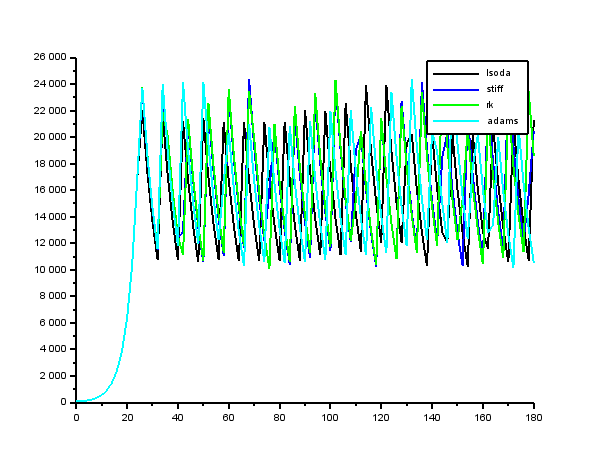
\includegraphics[width=0.7\linewidth]{./figures/state_discontinuity_sharp_sci}
	\caption{State Discontinuity in Scilab with sharp tolerances}
	\label{fig:state_discontinuity_sharp_scilab}
\end{figure}

Again, in Figure $\ref{fig:state_discontinuity_sharp_scilab}$ we can see that sharp tolerances are not enough to get the correct answers. The solution did improve as all the solvers seem to follow the correct pattern but none oscillate between 10000 and 25000 with clear peaks and troughs at those values respectively. For the time period between 0 to 30, they all seem reasonably on the same line but as we go further in time, all of the solutions diverge. We also note that none of them got the correct solution discussed in Section $\ref{subsection:state_with_event_detection}$.

\subsection{Why even sharp tolerances failed}
\label{subsection:state_sharp_tol_failed}
In this Section we discuss why sharp tolerances cannot solve the problem in the naive way it is coded, i.e using global variables and if-statements. 

This is because whenever there is a change in the value of $\beta$, the step that first encounters that change will always fail. As discussed in Section $\ref{subsection:effect_of_discontinuity}$, the step size at a discontinuity will always have to be much smaller than a step on a continuous region to be able to step over the discontinuity. Thus this first encounter will almost always be through too large a step and will fail. But in performing this step,  the value of the E inside the function will cross the threshold, especially if the method is using several stages, the global variables will thus be toggled as the codes inside the if-statement will run. But then when the solver will attempt to retake the step again and again, it will be using the wrong $\beta$ value. 

This observation is crucial as it allows us to conclude that at a discontinuity some of the function evaluations along the step should be using the old $\beta$ value while the others should be using the new $\beta$ value. There are no trivial way to code this behaviour in the ODE function, $f(t, y)$, if we do not know the time of the discontinuity.

At extremely sharp tolerances, even beyond $10^{-12}$, the first step that encounters the discontinuity can also fail. The solver will still have to retake the step but as shown, it will have to use wrong $\beta$ as there are no trivial way to code that some stages in that step should use the old one while some should use the new one. In the next sections, we will present the correct way to code problems with state dependent discontinuities so that we get the required behaviour.

\subsection{Introducing event detection}
\label{subsection:intro_event_detection}
In the time dependent problem, we saw that if we used error-controlled software, then the solvers can work through one discontinuity at sufficiently high tolerances. We also showed that with just one discontinuity, the problem could have been solved by sharper tolerances also but we showed that this was not the most efficient way to do so. In the previous section we showed why even sharp tolerances will not be able to solve this problem. However, the idea that we developed in Section $\ref{subsection:time_disc_handling}$ about integrating continuous sub-problems of the ODE separately and combining them into a final solution can still be applied here. 

To integrate continuous sub-problems, we only need a way to detect that the thresholds have been met and as soon as we see a threshold, we would cold start. This will make the solver integrate the problem one continuous subinterval at a time. In this Section, we will explain the capability of modern solvers to detect events and in the next Section, we will show how to encode the given thresholds as events to perform a cold start when they are reached.

An event in numerical ODE occurs whenever the solver detects a root of the function it is solving for. The solver will require two functions from the user as a result: the usual ODE right-hand side function, $f(t, y)$ and another function that defines how to look for the roots which we will call the root-function (commonly denoted by $g(t, y)$).

The root function is a function that given the value of the solution to the ODE at the current step will return a real number. The ODE solution is said to have a root whenever the value of the root-function is zero.

The solver calls the root-function at each step that it takes and will record its value. It will then compare the value of the root-function with the immediate previous value and see if there was a change of sign. If the value of the root-function changed sign, the solver raises a flag to say that it has detected a root and will then run a root-finding subroutine on that interval until it finds the exact point where the root-function returns zero. Most solvers will return the solution from that root and stop the integration, allowing us to cold start.

To use event detection thus entails defining a function that takes the value of the ODE solution at the current point and return a real number which is zero whenever we want it to detect an event. If we want to detect whenever x is 100, it is sufficient to return (x - 100) from the root-function. The next section will elaborate on how to use event detection for the state dependent discontinuity problem.

\subsection{Solving State discontinuity using event detection}
\label{subsection:state_with_event_detection}
Each toggling between the values of the parameter $\beta$ introduces a discontinuity. As none of the provided solvers are designed to solve discontinuous problems, we get the previously reported erroneous solution. We have seen that though sharp tolerances give better solutions, none of the solvers were along the same line and so the results were still wrong. Such sharp tolerances come with inefficiencies as well. We will now present a solution using event detection that is both accurate and efficient.

The solution is to use the thresholds that we have defined in our model as events and integrate only up to the first threshold we meet with each call to the solver. We can then cold start from there and repeat the process with another right hand side function denoting the new model and with another root-function which encodes the next threshold we are looking for.  As this new call meets its threshold, we repeat the process using the first ODE and root functions. We repeat this until we reach the end of the time interval. This solve continuous sub-problems one at a time and these sub-problems can then combined into a final solution. This strategy thus both avoid discontinuities and allows us to 'step' over the discontinuity with the function calls before it using the old parameters and the function calls after it using the new parameters.

For our specific problem, event detection is used as such:
We start by solving the problem with $\beta$ at 0.9 and with a root function that detects 25000. Once we detect 25000, we do a cold start. We extract the solution of the solver at the time of the event and use those values as the initial value for our next call to the solver. This next call will have $\beta$ at 0.005 and a root function that detects a root at 10000. We again integrate up to that new threshold and cold start when we reach it. The new cold start will have $\beta$ at 0.9 and the root function looking for 25000 as the event. This is repeated until we reach the desired end time.

The pseudo-code is as such:

\begin{minipage}{\linewidth}
\centering
\begin{lstlisting}[language=Python]
function model_no_measures(t, y):
    beta = 0.9
    // code to get dSdt, dEdt, dIdt, dRdt
    return (dSdt, dEdt, dIdt, dRdt)

function root_25000(t, y):
    E = y[1]
    return E - 25000

function model_with_measures(t, y):
    beta = 0.005
    // code to get dSdt, dEdt, dIdt, dRdt
    return (dSdt, dEdt, dIdt, dRdt)

function root_10000(t, y):
    E = y[1]
    return E - 10000

res = array()
t_initial = 0
y_initial = initial_values
while t_initial < 180:
    tspan = [t_initial, 180]
    if (measures_implemented):
        sol = ode(model_with_measures, tspan, y_initial,
         events=root_10000)
        measures_implemented = False
    else:
        sol = ode(model_no_measures, tspan, y_initial,
         events=root_25000)
        measures_implemented = True
    t_initial = extract_last_t_from_sol(sol)
    y_initial = extract_last_row_from_sol(sol)
    res = concatenate(res, sol)

// use res as the final solution
\end{lstlisting}
\end{minipage}

Some programming environments, such as Python, do not stop the integration as the first event is detected by default. To do a cold start, we need them to stop at events and thus when programming, we need to set the appropriate flags. (In Python, it is done by setting the terminal flag of the root functions. Example: $root\_10000.terminal = True$)

Each call to the solvers will have a continuous problem and thus will satisfy the requirements for their underlying theories. We will show that this is enough to get high accuracy efficient forecasts.  

\subsubsection{Solving state discontinuity in R}
\begin{figure}[h]
	\centering
	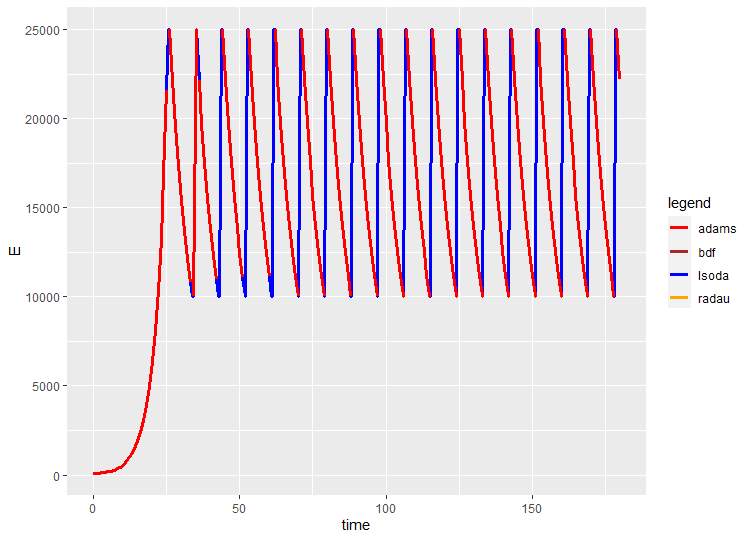
\includegraphics[width=0.7\linewidth]{./figures/solve_state_discontinuity_R}
	\caption{Solving state Discontinuity in R}
	\label{fig:solve_state_discontinuity_R}
\end{figure}
We note that only a few solvers have event detection capabilities in R. These are: adams, bdf, lsoda, radau. From Figure $\ref{fig:solve_state_discontinuity_R}$, we can see that all the solvers give solutions that are on the same line. This is in contrast with what happened previously when we were integrating a discontinuous problem, even at sharp tolerances. We will show in Table $\ref{tab:state_discontinuity_R}$ that introducing event detection also made the solvers significantly more efficient. 

We note that it is unfair to compare the efficiency at the default tolerances to the event detection's efficiency as their results were completely wrong. We can only compare the values with the sharp tolerance values.

\begin{table}[h]
\caption {R State Discontinuity problem} 
\label{tab:state_discontinuity_R}
\begin{center}
\begin{tabular}{ c c c c } 
    method & nfev & nfev sharp & event nfev \\ 
    lsoda &   2135    & 4658  & 1226  \\
    daspk &    5143   & 15185 & NaN   \\
    euler &    181   & 181   & NaN   \\
    rk4  &     721   & 721   & NaN   \\
    ode45 &    2027   & 18246 & NaN   \\
    radau &   1002    & 21835 & 2232  \\
    bdf   &   3300    & 9803  & 1657  \\
    adams &   1368    & 3467  & 802   \\
\end{tabular}
\end{center}
\end{table}

We can see from Table $\ref{tab:state_discontinuity_R}$ that even with sharp tolerances, we had inaccurate results and this required significantly more function evaluations. We note that we are gaining around 3000 function evaluations in 'lsoda', 20000 in 'radau', 8000 in 'bdf' and 2500 in 'adams' while having more accuracy. This significant decrease in the number of function evaluations will lead to much faster CPU times, especially when the right hand side function , $f(t, y)$ is a more complex function.

\subsubsection{Solving state discontinuity in Python}
\begin{figure}[h]
	\centering
	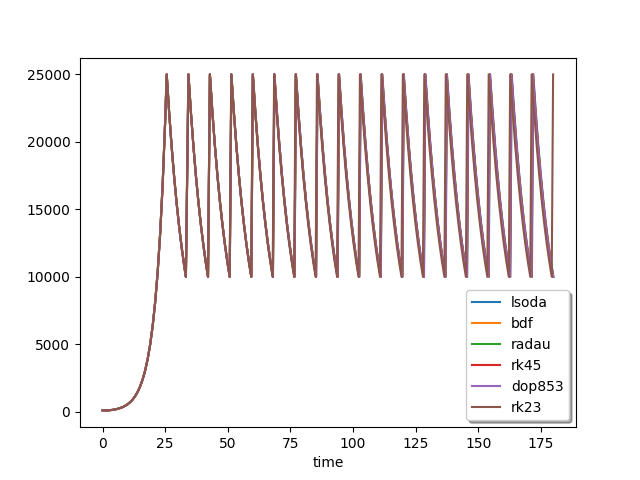
\includegraphics[width=0.7\linewidth]{./figures/solve_state_discontinuity_py}
	\caption{Solving state Discontinuity in Python}
	\label{fig:solve_state_discontinuity_py}
\end{figure}
All the solvers in Python have event detection. Again, Figure $\ref{fig:solve_state_discontinuity_py}$ shows that all the solvers give solutions that are on the same line, prompting that this is the correct solution. This is different from our results when integrating with a single $solve\_ivp()$ call. We will also see that this is much more efficient across all the solvers.

As in the case with R, we cannot compare the default tolerance efficiency data to the event detection efficiency data as the former clearly had worse results. So, in table $\ref{tab:state_discontinuity_Py}$, we compare the sharp tolerance efficiency data with the data from the event detection.

\begin{table}[h]
\caption {Python State Discontinuity problem} \label{tab:state_discontinuity_Py}
\begin{center}
\begin{tabular}{ c c c c } 
    method & nfev & nfev sharp & event nfev  \\ 
    lsoda  &   2357    &4282   & 535  \\
    bdf    &   2301   &11794  & 808  \\
    radau  &   211   &74723  & 990  \\
    rk45   &   1484   &17648  & 674  \\
    dop853 &   11129   &21131  & 1514 \\
    rk23   &   4307   &246644 & 589  \\
\end{tabular}
\end{center}
\end{table}

Table $\ref{tab:state_discontinuity_Py}$ shows that the number of function evaluations using event detection is far less; 'lsoda' used around 3000 less function evaluations, 'bdf' used 11000 less, radau used 74000 less, rk45 used 17000 less, 'dop853' used 20000 less and 'rk23' used 246000 less function evaluations. The reduction in CPU times from this will be significant across all the solvers, especially with a more complex right hand side function.

\subsubsection{Solving state discontinuity in Scilab}
\begin{figure}[h]
	\centering
	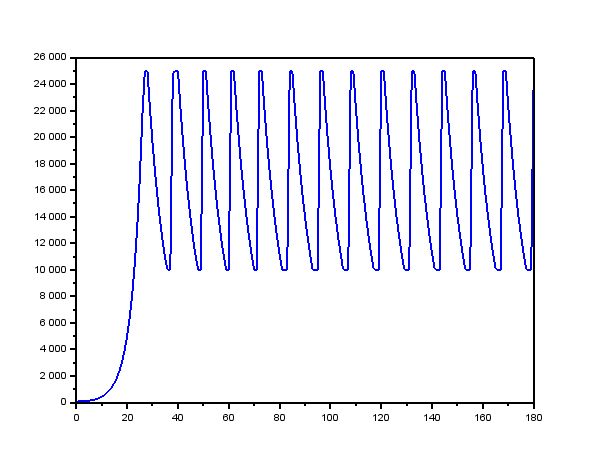
\includegraphics[width=0.7\linewidth]{./figures/solve_state_discontinuity_scilab}
	\caption{Solving state Discontinuity in Scilab}
	\label{fig:solve_state_discontinuity_scilab}
\end{figure}
There is only one solver with root functionality in Scilab which is the 'lsodar', the root-finding version of 'lsoda'. We do not get to compare it with other solvers but judging from the solutions we got from Python and R, it seems that it gave a correct solution as well. It is oscillating in the correct pattern and goes sharply between 10000 and 25000.

\begin{table}[h]
\caption {ScilabState Discontinuity problem} \label{tab:state_discontinuity_scilab}
\begin{center}
\begin{tabular}{ c c c c } 
method & nfev & nfev sharp & event nfev  \\ 
lsoda  & 2794.  & 4636.  & 1327. \\
stiff  & 3476.  & 9797.  & ---   \\
rkf    & 3004.  &  ---   & ---   \\
rk     & 12131. & 45940. & ---   \\
adams  & 2979.  & 5694.  & ---   \\
\end{tabular}
\end{center}
\end{table}

VI ===========
do you want me to add daskr
========== VI

\subsection{Efficiency data and tolerance Study for the state discontinuous problem}
\label{subsection:state_tolerance_study}
We can see that default tolerances for the model without event detection does not give correct answers. In this section, we will investigate how sharpening the tolerance improves the results in the case of the non-event detection experiment while we coarsen the tolerance with the event detection code to show how coarse a tolerance we can use while getting good results

We will perform this analysis on LSODA across R, Python and Scilab as they appear to use the same source code and with R's and Python's version of DOPRI5 which does not use the same code but do use the same Runge-Kutta pair and Scilab's version of RKF45 which is not the same code, nor the same pair but is a Runge-Kutta pair of the same order. 

\subsubsection{Comparing LSODA across platforms for state discontinuous problem}

In this section, we use R's version of LSODA at multiple tolerances to see how it acts at multiple tolerances. We set both the relative and the absolute tolerance to a particular value and analyse the solution.

We know that without event detection, LSODA does not work even at very sharp tolerances but we report on any strange behaviour from the code. We also would like to know how coarse we can set the tolerance to still have the event detection code work.

\subparagraph{state discontinuity LSODA tolerance study in R}

\begin{figure}[h]
	\centering
	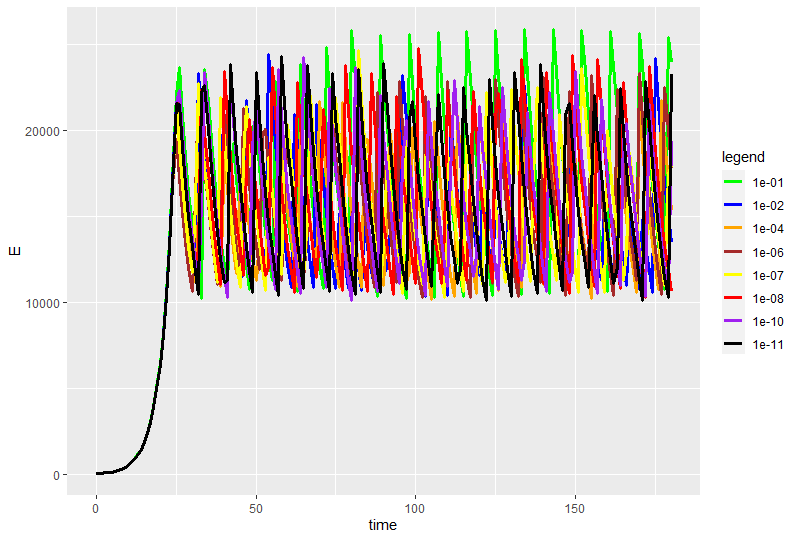
\includegraphics[width=0.7\linewidth]{./figures/tolerance_state_lsoda_no_event_R}
	\caption{State discontinuity tolerance study on R's LSODA without event detection}
	\label{fig:tolerance_state_lsoda_no_event_R}
\end{figure}

\begin{figure}[h]
	\centering
	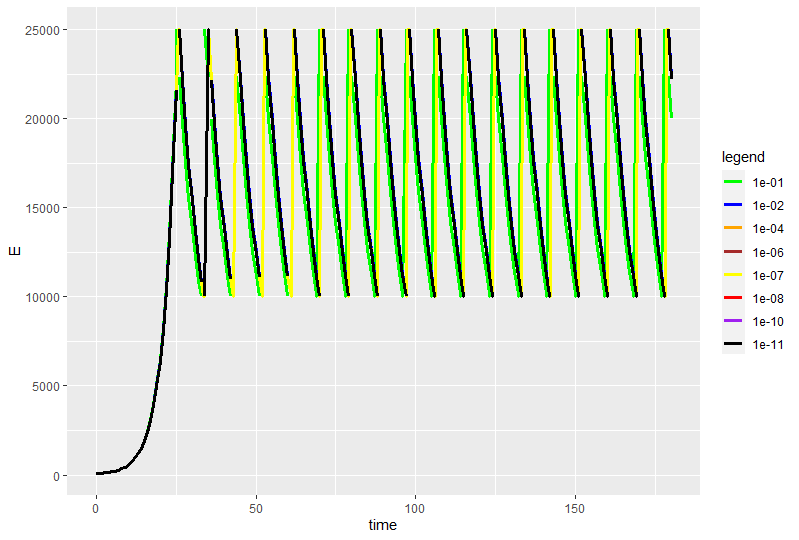
\includegraphics[width=0.7\linewidth]{./figures/tolerance_state_lsoda_with_event_R}
	\caption{State discontinuity tolerance study on R's LSODA with event detection}
	\label{fig:tolerance_state_lsoda_with_event_R}
\end{figure}

Figure $\ref{fig:tolerance_state_lsoda_no_event_R}$ shows a very strange behaviour. The same code with the same problem at different tolerances is giving vastly different results. We would expect the solutions at the sharper tolerances to be along very similar curves but that is not the case. We conclude that LSODA even at sharp tolerances is still resizing the step size. It is also suffering from the fact that the first step that encounters a discontinuity fails while still switching the global variables. This further proves our statement that for any state-dependent discontinuity, we cannot get the correct results simply by sharpening the tolerance.

From Figures $\ref{fig:tolerance_state_lsoda_with_event_R}$ and $\ref{fig:tolerance_state_lsoda_no_event_R}$, we can see the clear advantage of using event detection. Event detection even allows us to use very coarse tolerances while solving the problem correctly. Event detection allows us to use $10^{-3}$ and sharper to get the correct results while the code without event detection still failed at $10^{-13}$. We will also analyse the differences in efficiency between the two codes in Table $ref{tab:tolerance_state_discontinuity_lsoda_R}$.

\begin{table}[h]
\caption {R lsoda State Discontinuity tolerance study} \label{tab:tolerance_state_discontinuity_lsoda_R} 
\begin{center}
\begin{tabular}{ c c c c c }
tolerance & nfev & nsteps & event nfev & event nsteps \\ 
1e-01 &  675 &  274 &  552 &  233 \\
1e-02 & 1856 &  727 &  512 &  236 \\
1e-04 & 1863 &  706 &  736 &  350 \\
1e-06 & 2135 &  810 & 1226 &  559 \\
1e-07 & 2676 & 1005 & 1832 &  830 \\
1e-08 & 2730 & 1025 & 2032 &  911 \\
1e-10 & 3337 & 1392 & 2546 & 1212 \\
1e-11 & 3603 & 1566 & 2997 & 1470 \\
\end{tabular}
\end{center}
\end{table}

Table $\ref{tab:tolerance_state_discontinuity_lsoda_R}$ shows a decrease in the number of function evaluations which will translate into faster CPU times when the right hand side function is more complex. We note that the comparison is unfair as the code without event detection did not give a correct answer. However, it gave this wrong answer while still using more function evaluations which adds on to our conclusion that event detection is the correct way to solve state dependent discontinuity problems.

\subparagraph{discontinuity LSODA tolerance study in Python}
In this section, we use Python's version of LSODA at multiple tolerances to see how it performs. We set both the absolute and relative tolerance to a particular value. 

We note that LSODA without event detection even at very sharp tolerances in Python was still failing but we will see how the solutions change as the tolerance is increased. 

We will also show that coarse tolerances can be used with the code with event detection as each call to the solver is executing on continuous sub-intervals.   

\begin{figure}[h]
	\centering
	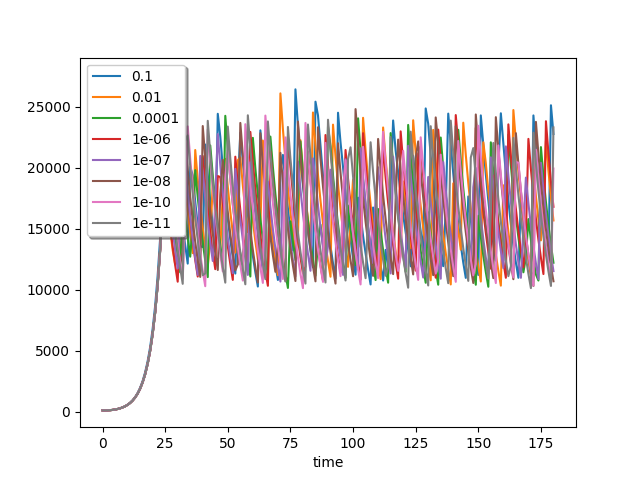
\includegraphics[width=0.7\linewidth]{./figures/tolerance_state_lsoda_no_event_py}
	\caption{State discontinuity tolerance study on Python's LSODA without event detection}
	\label{fig:tolerance_state_lsoda_no_event_py}
\end{figure}

\begin{figure}[h]
	\centering
	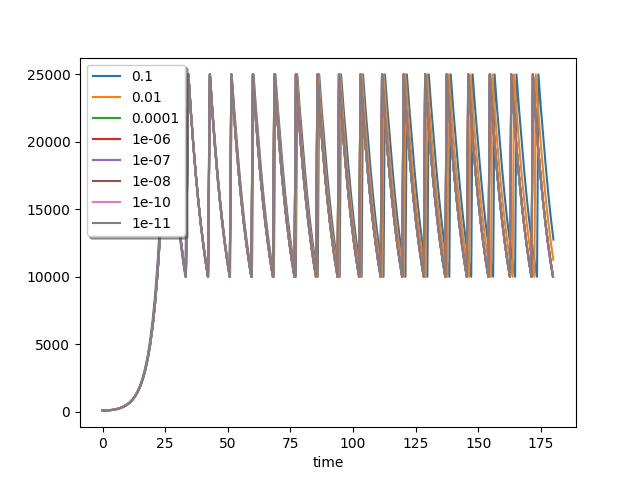
\includegraphics[width=0.7\linewidth]{./figures/tolerance_state_lsoda_with_event_py}
	\caption{State discontinuity tolerance study on Python's LSODA with event detection}
	\label{fig:tolerance_state_lsoda_with_event_py}
\end{figure}

Again Figure $\ref{fig:tolerance_state_lsoda_no_event_py}$ exposes the strange behaviour of LSODA whereby the same code with the same problem at different tolerances give different results. We would expect the code at the sharper tolerances to give very similar curves but clearly, LSODA even at sharp tolerances is still resizing the step size. This confirms that even at sharp tolerances, the step-size when first encountering the discontinuity is still too big. That first step will fail but will still switch the global variables. As a result, this problem cannot be solved by sharpening the tolerance.

From Figures $\ref{fig:tolerance_state_lsoda_with_event_py}$ and $\ref{fig:tolerance_state_lsoda_no_event_py}$, we can see that the addition of the event detection lets us use a smaller tolerance. We also note that the code with event detection blur as we go further in time. This is because the coarser tolerances are not giving the actual solution. In Python, it is at $10^{-4}$ and sharper that we are getting correct results. 

We then analyse the efficiency in Table $\ref{tab:tolerance_state_discontinuity_lsoda_py}$. We must note that this analysis is unfair as the code without event detection does not actually solve the problem. Still, we will see that the event detection code uses less function evaluations while getting the better answer.

\begin{table}[h]
\caption {Python LSODA State Discontinuity tolerance study} \label{tab:tolerance_state_discontinuity_lsoda_py} 
\begin{center}
\begin{tabular}{ c c c }
tolerance & nfev & event nfev \\ 
0.1    & 1207.0 & 425.0  \\
0.01   & 1627.0 & 454.0  \\
0.0001 & 1968.0 & 689.0  \\
1e-06  & 2122.0 & 1305.0 \\
1e-07  & 2684.0 & 1807.0 \\
1e-08  & 2730.0 & 2099.0 \\
1e-10  & 3337.0 & 2639.0 \\
1e-11  & 3603.0 & 3098.0 \\
\end{tabular}
\end{center}
\end{table}

Again we see in table $\ref{tab:tolerance_state_discontinuity_lsoda_py}$, that the code without event detection give us wrong answers while taking more function evaluations. A problem with a more complex right hand side function will take far less computational time with event detection than without.

\subparagraph{discontinuity LSODA tolerance study in Scilab}

We perform the same experiment in Scilab. We set the absolute and relative tolerance to the same particular value and run the solvers. For the different tolerance values, we plot the solutions and analyse how the solutions without event detection change as the tolerance is sharpened and how coarse a tolerance we can use with the event detection codes.

\begin{figure}[h]
	\centering
	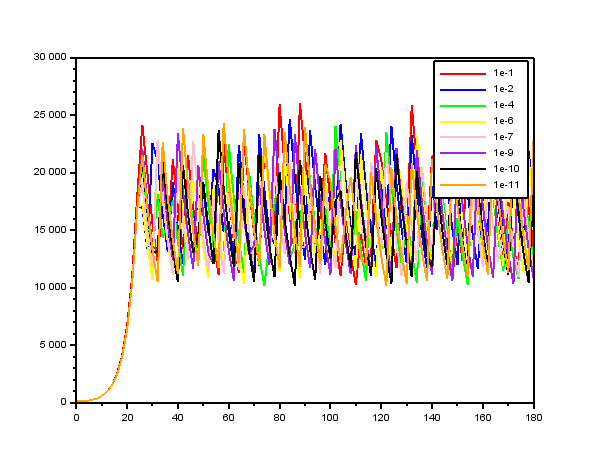
\includegraphics[width=0.7\linewidth]{./figures/tolerance_state_lsoda_no_event_sci}
	\caption{State discontinuity tolerance study on Scilab's LSODA without event detection}
	\label{fig:tolerance_state_lsoda_no_event_sci}
\end{figure}

\begin{figure}[h]
	\centering
	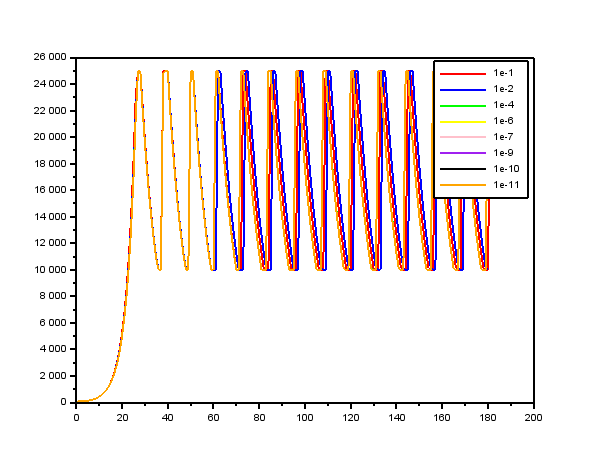
\includegraphics[width=0.7\linewidth]{./figures/tolerance_state_lsoda_with_event_sci}
	\caption{State discontinuity tolerance study on Scilab's LSODA with event detection}
	\label{fig:tolerance_state_lsoda_with_event_sci}
\end{figure}

Again, Figure $\ref{fig:tolerance_state_lsoda_no_event_sci}$ exposes the behaviour whereby the same code with the same problem at different tolerances give different results. We would expect the code at the sharper tolerances to give very similar curves but clearly, LSODA even at sharp tolerances is still resizing the step size. This confirms that even at high tolerances, the step-size when first encountering the discontinuity is still too big.

From Figures $\ref{fig:tolerance_state_lsoda_with_event_sci}$ and $\ref{fig:tolerance_state_lsoda_no_event_sci}$, the addition of the event detection lets us use a smaller tolerance. We also see that the code with event detection allows us to use a tolerance of $10^{-3}$ and still get the correct answer whereas without event detection, even a tolerance of $10^{-12}$ was not enough. 

\begin{table}[h]
\caption {Scilab LSODA State Discontinuity tolerance study} \label{tab:tolerance_state_discontinuity_lsoda_scilab} 
\begin{center}
\begin{tabular}{ c c c }
tolerance & nfev & event nfev \\ 
   0.1       & 1141.  & 287.  \\
   0.01      & 1606.  & 262.  \\
   0.0001    & 1968.  & 523. \\
   0.000001  & 2122.  & 983.  \\
   0.0000001 &  2684. & 1307.  \\
   1.000D-08 &  2730. & 1567. \\
   1.000D-10 &  3380. & 1963. \\
   1.000D-11 &  3603. & 2331. \\
\end{tabular}
\end{center}
\end{table}

\subsubsection{Comparing Runge-Kutta pairs across platforms for state discontinuous problem}

In this section, we use Runge-Kutta pairs of the same order; DOPRI5 in R aliased as 'ode45', DOPRI5 in Python aliased as 'RK45' and RKF45 in Scilab aliased as 'rkf'. 

We remember that without event detection, none of these solvers across the platforms solved the problem correctly even with sharp tolerances. We will show what happens to these code as the tolerance is sharpened to discuss why the problem is not solvable simply by sharpening the tolerance. We also coarsen the tolerance for the code with event detection where that is possible to see how coarse the tolerance can be while still obtaining sufficient accuracy.

\subparagraph{study on state discontinuity using R's DOPRI5}
R's DOPRI5 does not have event detection but we still perform the experiment on the code without event detection. We pick several values for the the absolute and relative tolerances and run the solvers. In so doing we see how the code performs as the tolerance is sharpened. 

\begin{figure}[h]
	\centering
	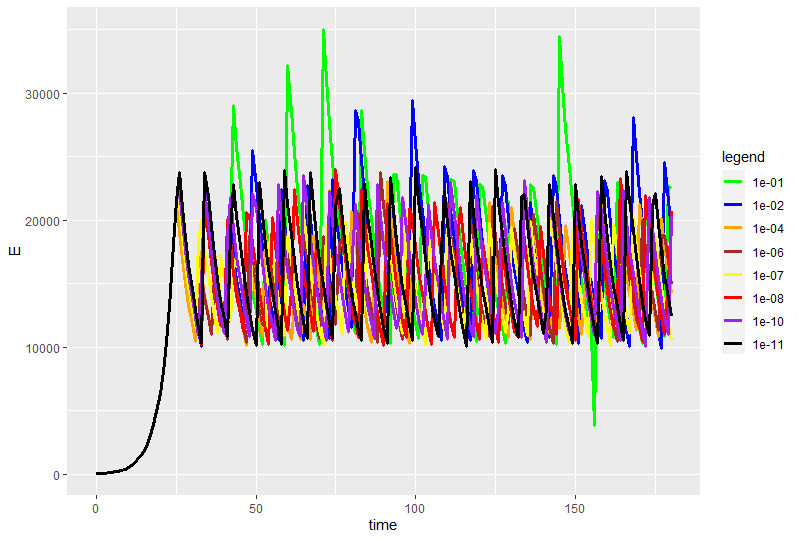
\includegraphics[width=0.7\linewidth]{./figures/tolerance_state_rk45_no_event_R}
	\caption{State discontinuity tolerance study on R's dopri5 without event detection}
	\label{fig:tolerance_state_rk45_no_event_R}
\end{figure}

Form Figure $\ref{fig:tolerance_state_rk45_no_event_R}$, we see the behaviour in LSODA whereby the same solver on the same problem with different tolerances still give different solutions. This tells us that the step is still being resized even at sharp tolerances and thus the first step that first encounters a discontinuity is still too big. The solver cannot step over the discontinuity and will have to repeatedly retake the step. But the global variables will be switched from the first step that encountered the discontinuity and thus the problem cannot be solved. This strengthens our conclusion that problem with similar state discontinuities cannot be solved without event detection.

We then report on the efficiency data with only the code without event detection in Table $\ref{tab:tolerance_state_discontinuity_rk45_R}$. 

\begin{table}[h]
\caption {R rk45 State Discontinuity tolerance study} \label{tab:tolerance_state_discontinuity_rk45_R} 
\begin{center}
\begin{tabular}{ c c c }
tolerance & nfev  & nsteps  \\ 
1e-01 & 1082 &  180 \\
1e-02 & 1142 &  189 \\
1e-04 & 2014 &  323 \\
1e-06 & 2027 &  328 \\
1e-07 & 2193 &  355 \\
1e-08 & 2919 &  471 \\
1e-10 & 5194 &  855 \\
1e-11 & 7690 & 1271 \\
\end{tabular}
\end{center}
\end{table}

\subparagraph{tolerance study on state discontinuity using Python's version of dopri5}
We perform the same experiment in Python. The absolute and relative tolerances is set to a particular value and the solver is run both with and without event detection. We report on how the code performs as the tolerance is increased in the case without event detection and as Python's version of DOPRI5 has event detection, we will see how coarse the tolerance can be set while still giving us a correct solution. 

\begin{figure}[h]
	\centering
	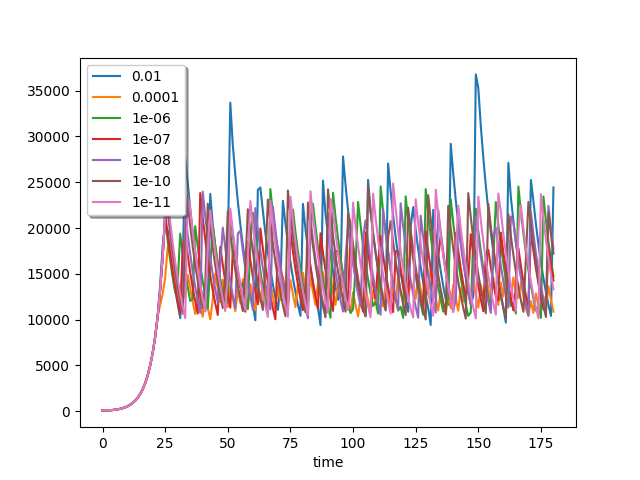
\includegraphics[width=0.7\linewidth]{./figures/tolerance_state_rk45_no_event_py}
	\caption{State discontinuity tolerance study on Python's DOPRI5 without event detection}
	\label{fig:tolerance_state_rk45_no_event_py}
\end{figure}

\begin{figure}[h]
	\centering
	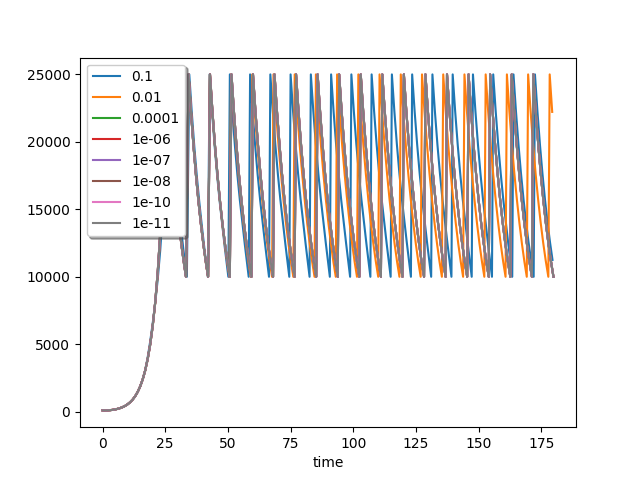
\includegraphics[width=0.7\linewidth]{./figures/tolerance_state_rk45_with_event_py}
	\caption{State discontinuity tolerance study on Python's DOPRI5 with event detection}
	\label{fig:tolerance_state_rk45_with_event_py}
\end{figure}

We must note that the solver crashes if we ask for a tolerance of 0.1 as it requires smaller steps in the case without event detection. The problem is too discontinuous and the solution is completely wrong as shown in Figure $\ref{fig:tolerance_state_rk45_no_event_0.1_py}$. The code stops at time 149 and cannot complete the whole time interval while getting a completely erroneous solution.

\begin{figure}[h]
	\centering
	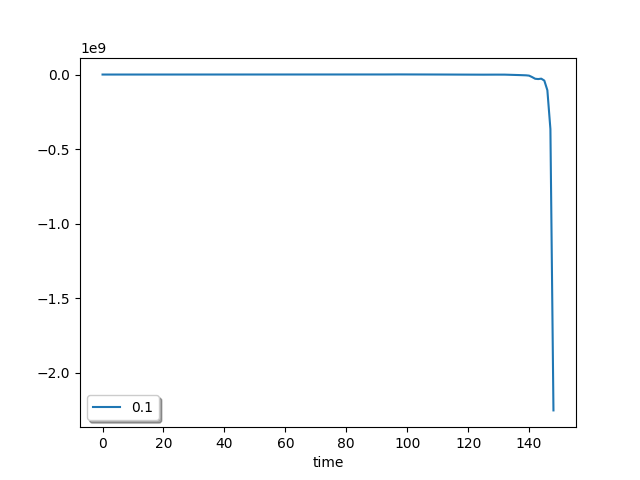
\includegraphics[width=0.7\linewidth]{./figures/tolerance_state_rk45_no_event_0.1_py}
	\caption{Python's DOPRI5 without event detection at 0.1 tolerances}
	\label{fig:tolerance_state_rk45_no_event_0.1_py}
\end{figure}

In Figure $\ref{fig:tolerance_state_rk45_no_event_py}$, we can see that even at sharp tolerances, the solver is still resizing the step-size. This indicates that even at sharp tolerances, the step along the continuous intervals are still bigger than at the discontinuity and the solver cannot step over it without resizing the step-size repeatedly. The global variables are switched at the first encounter with the discontinuity and thus the problem cannot be solved simply by increasing the tolerance.

In contrast, when using event detection, the code can use very coarse tolerances. We can see that $10^{-4}$ is sharp enough to solve the given problem, the blurring occurring due to the coarser tolerances. We then present the efficiency data in Table $\ref{tab:tolerance_state_discontinuity_rk45_py}$ to show how the code with event detection is also far more efficient.

\begin{table}[h]
\caption {Python rk45 State Discontinuity tolerance study} \label{tab:tolerance_state_discontinuity_rk45_py} 
\begin{center}
\begin{tabular}{ c c c }
tolerance & nfev & event's nfev  \\ 
0.1    & 536.0   & 664.0  \\
0.01   & 1400.0  & 664.0  \\
0.0001 & 8462.0  & 806.0  \\
1e-06  & 6248.0  & 1232.0 \\
1e-07  & 6848.0  & 1754.0 \\
1e-08  & 7082.0  & 2354.0 \\
1e-10  & 10262.0 & 5066.0 \\
1e-11  & 13058.0 & 7688.0 \\
\end{tabular}
\end{center}
\end{table}

We can see in Table $\ref{tab:tolerance_state_discontinuity_rk45_py}$ that across all the different tolerances except 0.1, the code with event detection require less function evaluations, around several thousands less for the sharper tolerances. We note that at a tolerance of 0.1, the code is using less function evaluations without event detection but at this tolerance, the code without event detection also gave a completely erroneous solution where it did not follow the oscillating between 10000 and 25000 pattern. 

\subparagraph{discontinuity RKF45 tolerance study in Scilab}
Scilab uses RKF45 which is a different Runge-Kutta pair as DOPRI5 but have the same order. It does not have event detection but we still perform the experiment on the code without event detection. We pick several values for the the absolute and relative tolerances and run the solvers. In so doing we see how the code performs as the tolerance is sharpened. 

Scilab's 'rkf' can only integrate up to time 90 as it has a hard cap of 3000 derivative evaluations but this is enough to see that even at sharper tolerances, the solutions are not on the same line. Figure $\ref{fig:tolerance_state_rk45_no_event_sci}$ shows that the step is still being resized and thus the problem cannot be solved by simply using higher tolerances. We can then conclude that event detection is required. 

\begin{figure}[h]
	\centering
	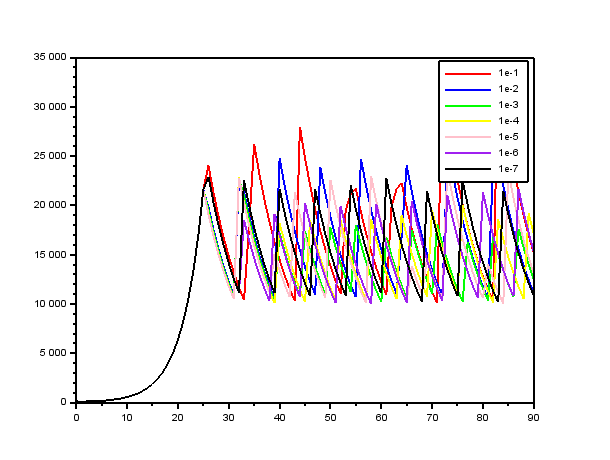
\includegraphics[width=0.7\linewidth]{./figures/tolerance_state_rk45_no_event_sci}
	\caption{State discontinuity tolerance study on Scilab's RKF45 without event detection}
	\label{fig:tolerance_state_rk45_no_event_sci}
\end{figure}

\begin{table}[h]
\caption {Scilab RKF45 State Discontinuity tolerance study} \label{tab:tolerance_state_discontinuity_rk45_scilab} 
\begin{center}
\begin{tabular}{ c c }
tolerance & nfev \\ 
   0.1    & 547. \\
   0.01   & 732. \\
   0.001  & 1294. \\
   1e-4   & 1956. \\
   1e-5   & 2364. \\
   1e-6   & 2662. \\
   1e-7   & 2802. \\
\end{tabular}
\end{center}
\end{table}
